\documentclass[../Report.tex]{subfiles}
\usepackage[italian]{babel}
\begin{document}
    \section{Random Forest}
    L'algoritmo \emph{Random Forest} o \emph{Random Decision Forest} è un algoritmo di classificazione e regressione che opera costruendo una moltitudine di alberi di decisione durante la fase di training. Per i task di classificazione l'output sarà la classe più selezionata dagli alberi. Per i task di regressione l'output sarà la media delle predizioni dei singoli task. In questo lavoro, essendo un lavoro di classificazione abbiamo utilizzato il \emph{RandomForestClassifier} di \emph{sckit-learn}.
    Il lavoro è stato organizzato in questo modo:
    \begin{enumerate}
        \item Utilizzando solo i dati personali degli utenti ed escludendo quelli degli esami superati e dei CFU raggiunti (il dataset bilanciato al momento dell'iscrizione, \ref{sec: balanced}) sono state provate varie modifiche dei parametri del modello, cambiando il dato relativo al \emph{numero di estimatori.}
        \item Successivamente, scelto il parametro che offre risultati migliori sono state provate diverse configurazioni del dataset. 
    \end{enumerate}
    Nella prima fase del lavoro siamo andati quindi a valutare quanto il cambiamento degli iperparametri del modello incidessero sui risultati. Avendo notato come il parametro che incidesse di più sul cambiamento dei risultati sia \emph{n\_estimators} e avendo notato come il variare di altri parametri quali \emph{max\_depth, min\_samples\_leaf} incidano poco sul risultato, per motivi di potenza di calcolo, abbiamo preferito effettuare il tuning solo sull'iperparametro n\_estimators. Per prima cosa eravamo interessati a vedere di quanto potesse variare l'accuratezza al variare del parametro. Abbiamo, quindi, costruito un  grafico che mette in relazione l'accuratezza al numero di estimatori  nel modello. I tentativi di calcolare questo rapporto anche fino a valori molto alti fallivano a causa di esecuzioni troppo lunghe per la nostra potenza di calcolo. Per avere un'idea del fenomeno siamo andati quindi a calcolare l'accuracy in base al numero di alberi per tutti i valori da uno a cinquecento. Mostriamo ora il grafico ottenuto:
    \begin{figure}[H]
        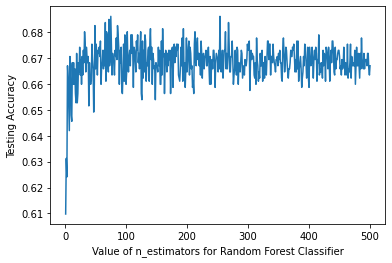
\includegraphics[width=0.7\linewidth]{../../Images/AccuracyvsNestimatorns.png}
        \centering
    \end{figure}
    Come si può notare dal grafico piccole variazioni del parametro possono far variare il risultato di accuratezza ottenuto. 
    Ci siamo chiesti quindi se valori molto piu grandi di questo iperparametro potessero cambiare sensibilmente la situazione. Abbiamo utilizzato in questo caso, il metodo \emph{GridSearchCV}. Tramite questo metodo è possibile definire una griglia di valori di iperparametri sui quali randomicamente verrà fatto train e test di un modello applicando una k-fold cross validation. La ricerca è stata effettuata sui valori da 1 a 500 e su 1000, 10000, 50000, 100000 con un \emph{k} pari a 3. Alla fine dell'esecuzione abbiamo stampato quindi il valore di \emph{best\_params\_} che è risultato pari a 207. È stato quindi utilizzato sempre questo come parametro in tutti i modelli creati successivamente. Per garantire, inoltre, una riproducibilità dei risultati è stato impostato un \emph{RandomState} pari a 42.
    \begin{figure}[H]
        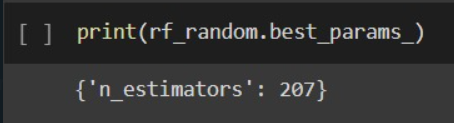
\includegraphics[width=0.7\linewidth]{../../Images/bestparamsRF.png}
        \centering
    \end{figure}
\end{document}